%%%%%%%%%%%%%%%%%%%%%%%%%%%%%%%%%%%%%%%%%
% Journal Article
% LaTeX Template
% Version 1.4 (15/5/16)
%
% This template has been downloaded from:
% http://www.LaTeXTemplates.com
%
% Original author:
% Frits Wenneker (http://www.howtotex.com) with extensive modifications by
% Vel (vel@LaTeXTemplates.com)
%
% License:
% CC BY-NC-SA 3.0 (http://creativecommons.org/licenses/by-nc-sa/3.0/)
%
%%%%%%%%%%%%%%%%%%%%%%%%%%%%%%%%%%%%%%%%%

%----------------------------------------------------------------------------------------
%	PACKAGES AND OTHER DOCUMENT CONFIGURATIONS
%----------------------------------------------------------------------------------------

\documentclass[twoside]{article}

\usepackage{blindtext} % Package to generate dummy text throughout this template 

\usepackage[sc]{mathpazo} % Use the Palatino font
\usepackage[T1]{fontenc} % Use 8-bit encoding that has 256 glyphs
\linespread{1.05} % Line spacing - Palatino needs more space between lines
\usepackage{microtype} % Slightly tweak font spacing for aesthetics

\usepackage[english]{babel} % Language hyphenation and typographical rules

\usepackage[a4paper, hmarginratio=1:1,top=32mm,columnsep=20pt]{geometry} % Document margins
\usepackage[hang, small,labelfont=bf,up,textfont=it,up]{caption} % Custom captions under/above floats in tables or figures
\usepackage{booktabs} % Horizontal rules in tables

\usepackage{lettrine} % The lettrine is the first enlarged letter at the beginning of the text

\usepackage{enumitem} % Customized lists
\setlist[itemize]{noitemsep} % Make itemize lists more compact

\usepackage{abstract} % Allows abstract customization
\renewcommand{\abstractnamefont}{\normalfont\bfseries} % Set the "Abstract" text to bold
\renewcommand{\abstracttextfont}{\normalfont\small\itshape} % Set the abstract itself to small italic text

\usepackage{titlesec} % Allows customization of titles
\renewcommand\thesection{\Roman{section}} % Roman numerals for the sections
\renewcommand\thesubsection{\roman{subsection}} % roman numerals for subsections
\titleformat{\section}[block]{\large\scshape\centering}{\thesection.}{1em}{} % Change the look of the section titles
\titleformat{\subsection}[block]{\large}{\thesubsection.}{1em}{} % Change the look of the section titles

\usepackage{fancyhdr} % Headers and footers
\pagestyle{fancy} % All pages have headers and footers
\fancyhead{} % Blank out the default header
\fancyfoot{} % Blank out the default footer
\fancyhead[L]{Ryan Cox} % Custom header text
\fancyhead[C]{April 2022} 
\fancyhead[R]{PHYS415}
\fancyfoot[RO,LE]{\thepage} % Custom footer text

\usepackage{titling} % Customizing the title section

\usepackage{hyperref} % For hyperlinks in the PDF

% Packages added by me, not from templates
\usepackage{amsmath}
\usepackage{graphicx}
\graphicspath{ {./images/} }
\usepackage[separate-uncertainty=true]{siunitx}
\usepackage{multirow}
\usepackage{tabularx}
\newcolumntype{R}{>{\raggedleft\arraybackslash}X}
\usepackage{physics}
\usepackage{stfloats}

\usepackage{csquotes}
\usepackage[style=phys]{biblatex}
\addbibresource{bib.bib}

\setlength {\marginparwidth }{2cm}
\usepackage{todonotes}


\hypersetup{
  colorlinks   = true, %Colours links instead of ugly boxes
  urlcolor     = blue, %Colour for external hyperlinks
  linkcolor    = blue, %Colour of internal links
  citecolor   = red %Colour of citations
}

\newcommand\blfootnote[1]{%
  \begingroup
  \renewcommand\thefootnote{}\footnote{#1}%
  \addtocounter{footnote}{-1}%
  \endgroup
}

%----------------------------------------------------------------------------------------
%	TITLE SECTION
%----------------------------------------------------------------------------------------

\setlength{\droptitle}{-4\baselineskip} % Move the title up

\pretitle{\begin{center}\Huge\bfseries} % Article title formatting
\posttitle{\end{center}} % Article title closing formatting
\title{The Boris Method} % Article title
\author{%
\textsc{Ryan Cox} \\[1ex] % Your name
\normalsize PHYS 415: Electromagnetism\\ % Your institution
%\and % Uncomment if 2 authors are required, duplicate these 4 lines if more
%\textsc{Jane Smith}\thanks{Corresponding author} \\[1ex] % Second author's name
%\normalsize University of Utah \\ % Second author's institution
%\normalsize \href{mailto:jane@smith.com}{jane@smith.com} % Second author's email address
}
\date{\today} % Leave empty to omit a date

%----------------------------------------------------------------------------------------

\begin{document}

% Print the title
\maketitle

\tableofcontents

\section{Theory}

The motion of a charged particle subject subject only to forces from electric and magnetic fields is governed by the Newton-Lorentz force law
\begin{equation} \label{eq: lorentz}
    m\vb{a} = q(\vb{E}+\vb{v}\cp\vb{B})
\end{equation}

Given an initial position $\vb{r}(t_0)$ and velocity $\vb{v}(t_0)$ we can increment the time in small steps $\Delta t$. The most basic process of going from $t$ to $t+\Delta t$ is
\begin{enumerate}
    \item Update position $\vb{r}$ as $\vb{r}(t+\Delta t) = \vb{r}(t) + \vb{v}(t)\Delta t$
    \item Update velocity $\vb{v}$ as $\vb{v}(t+\Delta t) = \vb{v}(t) + \vb{a}(t)\Delta t$ where $\vb{a}(t)$ is derived from \autoref{eq: lorentz}
\end{enumerate}
Repeating this many time approximates the particle motion over a given period. However, this method has some significant drawbacks that cause its numerical solution to rapidly diverge from the analytical solution.

Firstly, it assumes $\vb{E}$ and $\vb{B}$ are constant across the distance traversed each iteration, giving constant acceleration over each step. We can approximate this scenario by choosing a small timestep.

Secondly, it calculates particle displacement from $t$ to $t+\Delta t$ by using the velocity at time $t$. It is easy to see that this leads to an inaccurate result when any significant acceleration is present. This can be corrected by using the average velocity over that step. As we assume constant acceleration each step this average is given by
\begin{equation}
    \frac{\vb{v}(t+\Delta t)+\vb{v}(t-\Delta t)}{2} = \vb{v}(t+\frac{\Delta t}{2})
\end{equation}
This method can be easily implemented by stepping the initial velocity $\vb{v}(t_0)$ back in time by $\Delta t/2$. This causes all future velocity steps to be correctly offset. We call this the leapfrog method.\cite{velocityintegration}

While this works well for the electric force, it is inaccurate for the magnetic force as it depends on velocity. We want to calculate the velocity as
\begin{equation} \label{eq: b correct v}
  \vb{v}(t+\frac{\Delta t}{2}) = \vb{v}(t-\frac{\Delta t}{2}) + \frac{q}{m} \left(\vb{E} + \vb{v_a}(t_i) \cp \vb{B})
    \right)
\end{equation}
where
\begin{equation} \label{eq: v avg}
  \vb{v_a}(t) = \frac{\vb{v}(t+\frac{\Delta t}{2})+\vb{v}(t-\frac{\Delta t}{2})}{2}
\end{equation}

The Boris method is a computationally efficient solution to this equation. First we define new vectors such that
\begin{equation} \label{eq: v minus}
  \vb{v}(t-\frac{\Delta t}{2}) = \vb{v^-} - \frac{q\vb{E}}{m}\frac{\Delta t}{2}
\end{equation}
\begin{equation} \label{eq: v plus}
  \vb{v}(t+\frac{\Delta t}{2}) = \vb{v^+} + \frac{q\vb{E}}{m}\frac{\Delta t}{2}
\end{equation}
Using this, \autoref{eq: v avg} and \autoref{eq: b correct v} we find
\begin{equation}
  \frac{\vb{v^+}-\vb{v^-}}{\Delta t} = \frac{q}{2m}\left(\vb{v^+}+\vb{v^-}\right)\cp\vb{B}
\end{equation}
By geometric arguments\cite{Birdsall1991} we can define additional vectors such that
\begin{equation}
  \vb{v\prime} = \vb{v^-} + \vb{v^-} \cp \vb{t}
\end{equation}
\begin{equation}
  \vb{v^+} = \vb{v^-} + \vb{v\prime} \cp \vb{s}
\end{equation}
where
\begin{equation}
  \vb{t} \equiv \frac{q\vb{B}}{m}\frac{\Delta t}{2}
\end{equation}
\begin{equation}
  \vb{s} \equiv \frac{2\vb{t}}{1+t^2}
\end{equation}
Thus we can proceed along the chain
\begin{equation} \label{eq: boris process}
  \vb{v}(t-\frac{\Delta t}{2}) \to
  \vb{v^-} \to
  \vb{v\prime} \to
  \vb{v^+} \to
  \vb{v}(t+\frac{\Delta t}{2})
\end{equation}
In effect, we apply half the electric force, rotate the velocity vector due to the magnetic field and then apply the rest of the electric force.\cite{vxbrotation}

Using this method to update velocity in our leapfrog method gives us the Boris method. It is efficient to compute and remains accurate for long periods.

\section{Results}
From the plots it can be seen that the numerical and analytical methods agree within a reasonable margin over 1000 iterations with timestep \SI{3e-11}{\second}.

\begin{figure}
  \centering
  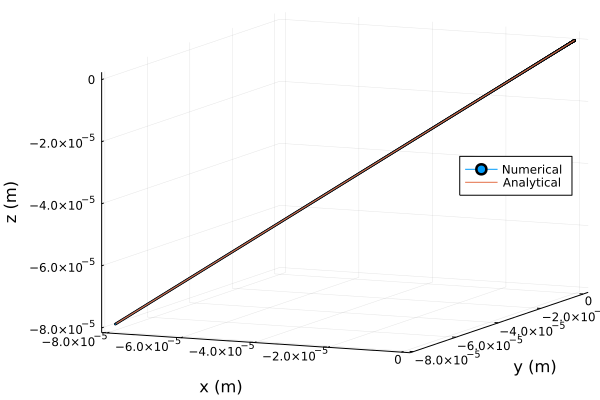
\includegraphics[width=\textwidth]{Econst_B0.png}
  \caption{$\vb{E}=(1,1,1)\si{\volt\per\metre}$, zero magnetic field and initial velocity, initial position at origin.}
  \label{fig: E const B 0}
\end{figure}
\begin{figure}
  \centering
  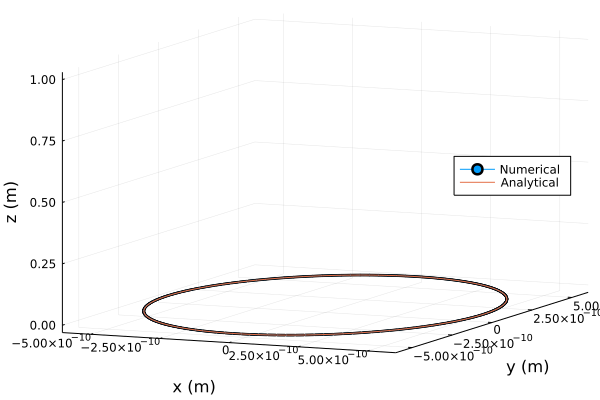
\includegraphics[width=\textwidth]{E0_Bconst.png}
  \caption{$\vb{B}=(0,0,0.01)\si{\tesla}$, zero electric  field, initial velocity $(0, 1, 0)\si{\metre}$, initial position $(5.686017478152309\times10^{-10}, 0, 0)\si{\metre}$.}
  \label{fig: E 0 B const}
\end{figure}
\begin{figure}
  \centering
  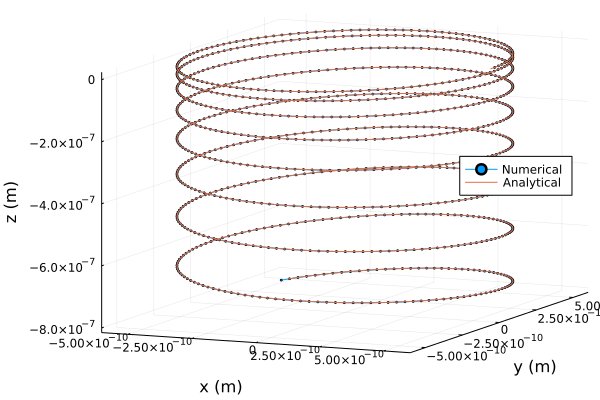
\includegraphics[width=\textwidth]{Econst_Bconst.png}
  \caption{$\vb{E}=(0,0,0.01)\si{\volt\per\metre}$, $\vb{B}=(0,0,0.01)\si{\tesla}$, initial velocity $(0, 1, 0)\si{\metre}$, initial position $(5.686017478152309\times10^{-10}, 0, 0)\si{\metre}$.}
  \label{fig: E const B const}
\end{figure}
\begin{figure}
  \centering
  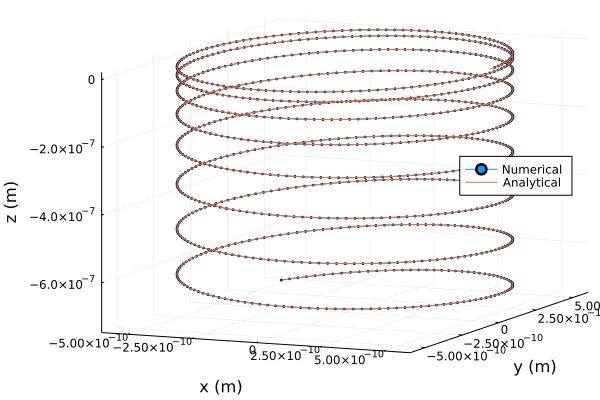
\includegraphics[width=\textwidth]{Epartial_Bconst.png}
  \caption{$\vb{E}=(0,0,0.01)\si{\volt\per\metre}$ when $z>\SI{-4e-7}{\metre}$, $\vb{B}=(0,0,0.01)\si{\tesla}$, initial velocity $(0, 1, 0)\si{\metre}$, initial position $(5.686017478152309\times10^{-10}, 0, 0)\si{\metre}$.}
  \label{fig: E partial B const}
\end{figure}

\printbibliography


%----------------------------------------------------------------------------------------

\end{document}
